\section{Beispiele}

In diesem Abschnitt werden verschiedene Berechnungsbeispiele aufgeführt.


\subsection{Berechnung der Entropie einer Quelle mit Gedächtnis}

Eine Quelle mit GEdächtnis kann mit einem Markoff-Diagramm dargestellt werden.
Diese Überlegungen und Berechnungen gelten auch für das Kanalmodell.

Bei Quellen mit Gedächtnis können wir ahnen, welches Zeichen als nächstes kommt,
daher sinkt der Informationsgehalt und die Redundanz nimmt zu.

\begin{tikzpicture}[->,>=stealth',shorten >=1pt,auto,node
                    distance=2.8cm,semithick]

	\node[state] (A)                    {$A$};
	\node[state] (B) [below left of=A]  {$B$};
	\node[state] (C) [below right of=A] {$C$};

	\path (A) edge [bend right] node [above left]  {$\sfrac{4}{5}$}  (B)
	          edge [bend left]  node               {$\sfrac{1}{5}$}  (C)
	      (B) edge [bend right] node [below right] {$\sfrac{1}{2}$}  (A)
	          edge [loop below] node               {$\sfrac{1}{2}$}  (B)
	      (C) edge [bend left]  node               {$\sfrac{1}{2}$}  (A)
	          edge [bend left]  node               {$\sfrac{2}{5}$}  (B)
	          edge [loop below] node               {$\sfrac{1}{10}$} (C)
	;

\end{tikzpicture}



\subsubsection*{1. Aufstellen der Matrix für die bedingte Wahrscheinlichkeit}

Die Werte können aus dem Diagramm ausgelesen werden.

\begin{tabular}[H]{|c|c|c|c|c|}
	\hline
	$p(y|x)$ & $Y=$ & $A$ & $B$ & $C$ \\
	\hline
	\multirow{3}{*}{$X=$} & $A$ geht über in & $0$ & $\frac{4}{5}$ & $\frac{1}{5}$ \\
	\cline{2-5}
	& $B$ geht über in & $\frac{1}{2}$ & $\frac{1}{2}$ & $0$ \\
	\cline{2-5}
	& $C$ geht über in & $\frac{1}{2}$ & $\frac{2}{5}$ & $\frac{1}{10}$ \\
	\hline
\end{tabular}


\subsubsection*{2. Berechnen der Wahrscheinlichkeit der einzelnen Zeichen}

Aufstellen der vier Gleichungen:

% TODO unterschied P vs p?
\begin{equation*}
	\begin{array}{rclclcl}
		1    &=& p(A)                   &+& p(B)                   &+& p(C) \\
		p(A) &=& p(A) \cdot 0           &+& p(B) \cdot \frac{1}{2} &+& p(C) \cdot \frac{1}{2} \\
		p(B) &=& p(A) \cdot \frac{4}{5} &+& p(B) \cdot \frac{1}{2} &+& p(C) \cdot \frac{2}{5} \\
		p(C) &=& p(A) \cdot \frac{1}{5} &+& p(B) \cdot 0           &+& p(C) \cdot \frac{1}{10}
	\end{array}
\end{equation*}

Daraus ergibt sich:
\begin{align*}
	p(A) &= \frac{1}{3} \\
	p(B) &= \frac{16}{27} \\
	p(C) &= \frac{2}{27}
\end{align*}


\subsubsection*{3. Zusammenfassen}

% TODO hä???
\begin{tabular}[H]{|c|c|c|c|c|}
	\hline
	$p(y|x)$ & $Y=$ & $A$ & $B$ & $C$ \\
	\hline
	\multirow{3}{*}{$X=$} & $A = \frac{1}{3}$ & $0 = 0$ & $\frac{4}{5} = \frac{4}{15}$ & $\frac{1}{5} = \frac{1}{15}$ \\
	\cline{2-5}
	& $B = \frac{16}{27}$ & $\frac{1}{2} = \frac{8}{27}$ & $\frac{1}{2} = \frac{8}{27}$ & $0 = 0$ \\
	\cline{2-5}
	& $C = \frac{2}{27}$ & $\frac{1}{2} = \frac{1}{27}$ & $\frac{2}{5} = \frac{4}{135}$ & $\frac{1}{10} = \frac{1}{135}$ \\
	\hline
\end{tabular}


\subsubsection*{4. Informationsgehalt der Zeichen}

Der Informationsgehalt berechnet sich wie folgt:
\[
	I(X_k) = \log_2\left(\frac{1}{p(x_k)}\right)
\]

Daraus ergibt sich:
{%
	\renewcommand{\arraystretch}{2}
	\begin{equation*}
		\begin{array}{rclcl}
			I(A) &=& \log_2\left(\frac{1}{\sfrac{1}{3}}\right) &=& 1.585 \, \textrm{Bit} \\
			I(B) &=& \log_2\left(\frac{1}{\sfrac{16}{27}}\right) &=& 0.755 \, \textrm{Bit} \\
			I(C) &=& \log_2\left(\frac{1}{\sfrac{2}{27}}\right) &=& 3.755 \, \textrm{Bit}
		\end{array}
	\end{equation*}
}%


\subsection{LZ78 Kompression}
\label{example:lz78}

Zu codierende Zeichenfolge: $00101110010110$

\subsubsection*{1. Aufteilen in eindeutige Zeichenfolgen}

\[
	0|01|011|1|00|10|11|0
\]

\subsubsection*{2. Übertragen}

\begin{minipage}{.4\linewidth}
	\begin{tabular}[H]{|l|l|}
		\hline
		0 & (0,0) \\
		\hline
		01 & (1,1) \\
		\hline
		011 & (2,1) \\
		\hline
		1 & (0,1) \\
		\hline
		00 & (1,0) \\
		\hline
		10 & (4,0) \\
		\hline
		11 & (4,1) \\
		\hline
		0 & (1) \\
		\hline
	\end{tabular}
\end{minipage}
\begin{minipage}{.6\linewidth}
	\tikzset{
	node/.style = {circle, draw=black, fill=white},
}

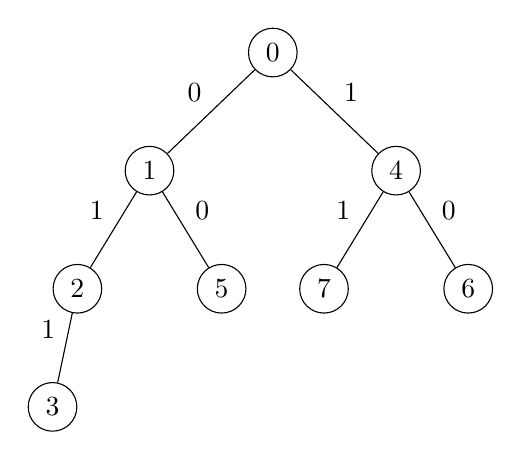
\begin{tikzpicture}
	\tikzstyle{level 1}=[sibling distance=25mm] 
	\tikzstyle{level 2}=[sibling distance=12mm] 
	\node[node]{0}
		child {
			node[node,left]{1}
			child {
				node[node,left]{2}
				child {
					node[node,left]{3}
					edge from parent node [above left] {1}
				}
				edge from parent node [above left] {1}
			}
			child {
				node[node,right]{5}
				edge from parent node [above right] {0}
			}
			edge from parent node [above left] {0}
		}
		child {
			node[node,right]{4}
			child {
				node[node,left]{7}
				edge from parent node [above left] {1}
			}
			child {
				node[node,right]{6}
				edge from parent node [above right] {0}
			}
			edge from parent node [above right] {1}
		}
	;
\end{tikzpicture}

\end{minipage}

\subsubsection*{3. Decodieren}

Bei jedem ankommenden Zeichenpaar wird der Baum bis zum entsprechenden Knoten
verfolgt und die Bits auf dem Weg ausgegeben. Danach wird bei Bedarf ein neuer
Knoten in den Baum eingefügt.

Beispiel (2,0):
\begin{itemize}
	\item Verfolgen des Baumes bis Knoten 2
	\item Ausgabe der Bits: $01$
	\item Anfügen eines neuen Knotens und Ausgabe des Weges dorthin: $0$
	\item Gesamte Bitfolge ist: $010$
\end{itemize}


\subsection{RSA}
\label{example:rsa}

Mit zwei Primzahlen und der Zahl $e$ kann man ein Schlüsselpaar bilden. Mit dem
Paar $(e,N)$ kann man eine Zahl verschlüsseln. Mit $(d,N)$ kann man sie
entschlüsseln.
\begin{description}
\item[Gegeben:] Primzahlen $p=11$ und $q=7$ und die Zahl $e$
\item[Gesucht: ] Schlüsselpaare für RSA
\end{description}
Zuerst muss $N$ berechnet werden:
\[
N = p*q
\]
\[
77 = 11*7
\]
Damit hat man schon ein Teil des Schlüssels $(e,N)$. Jetzt muss man noch die
Zahl $d$ für den zweiten Schlüssel $(d,N)$ berechnen. Für $d$ muss gelten $e*d
mod \phi(N) = 1$. Für die weiteren Schritte wird die Zahl $\phi(N)$ benötigt.
\[
\phi(N) = (p-1) * (q-1)
\]
\[
60 = (11-1) * (7-1)
\]
Um die Zahl $d$ für den zweiten Schlüssel herauszufinden muss man das ggT von
$\phi(N)$ und $e$ berechnen. Das ist logischerweise 1. Man möchte aber nicht das
ggT herausfinden, sondern man benötigt die Gleichungen des euklidischen
Algorithmus. Zuerst multipliziert man $e$ damit das Produkt $\leq \phi(N)$ ist
und addiert die Differenz $n$
\[
\phi(N) = k * e + n
\]
Bei der nächsten Gleichung setzt man für $\phi(N)$ $e$ ein und für $e$ $n$.
Irgendwann wird $n=0$ und $e=1$. Das wäre eigentlich das ggT. Das haben wir zwar
schon vorher gewusst. Man benötigt aber die Zwischenschrite. Mit Zahlen:
\begin{eqnarray}
\label{eqn:inv3}
60 & = & 8 * 7 + 4 \\
\label{eqn:inv2}
7 & = & 1 * 4 + 3\\
\label{eqn:inv1}
4 & = & 1 * 3 + 1\\
3 & = & 3 * 1 + 0
\end{eqnarray}
Die letzte Gleichung braucht man eigentlich nicht. Die letzte Gleichung
\ref{eqn:inv1} kann geschrieben werden als:
\begin{equation}
\label{eqn:subs}
1 = 4 - 1*3
\end{equation}
Gleichung \ref{eqn:inv2} kann als
\[
3 = 7 - 1*4
\]
geschrieben werden.
Mit \ref{eqn:inv2} kann die Zahl 3 in \ref{eqn:subs} ersetzt werden.  
\begin{equation}
1 = 4 - 1*(7-1*4)
\end{equation}
Diese Gleichung muss man so umformen, dass die Zahl 4 ein Faktor des zweiten
Summand ist, damit man sie danach wieder substituieren kann.
\begin{align}
1 &= 4 - 7+4 \\
1 &= -7 + 2*4
\end{align}
Die Zahl 4 substituiert mit Gleichung \ref{eqn:inv3} substituiert ergibt
\begin{equation}
1 = -7 + 2*(60-8*7)
\end{equation}
Diese Gleichung muss jetzt so umformen dass man etwas in der Form
\begin{equation*}
1 = 60*k + 7*d
\end{equation*}
oder
\begin{equation*}
1 = \phi*k + e*d
\end{equation*}
erhält. Weil damit ist die Bedingung $e*d \bmod \phi(N) = 1$ erfüllt.
\begin{eqnarray}
1 & = & -7 + 2*60-16*7 \\
1 & = & 2 * 60-16*7-7 \\
1 & = & 2 * 60-16*7-1*7\\
1 & = & 2 * 60-7(16+1)\\
1 & = & 2 * 60-17*7
\end{eqnarray}
Wenn $d$ negativ ist muss man noch $d \bmod N$ rechnen. Also $\unaryminus 17
\bmod 60 = 43$.  Somit ist $d = 43$
